\subsubsection{向量场在曲线上的积分的定义和计算}

% 20260512

$$\int_L\overrightarrow{v}\,\mathrm{d}\overrightarrow{r}\quad\int_{(L,O)}\overrightarrow{v}\,\mathrm{d}\overrightarrow{r}$$

\subparagraph*{Computation}

Take an ``\emph{oriented parametrization}'' $\overrightarrow{r}:\,[a,b]\to L$ (meaning $\underset{\overrightarrow{r}'(t)\cdot\left.\overrightarrow{\tau}\right|_{S\left(\overrightarrow{r}(t)\right)}}{\overrightarrow{r}'(t)}$ represents the given orientation)

\emph{An orientation is equivalent to a choice of continuous unit tangent vector field $\left\{\overrightarrow{\tau}(s)\right\}_{S\in[0,l]}$}

\begin{align*}
    \int_L\overrightarrow{v}\,\mathrm{d}\overrightarrow{r}
     & =\lim_{\|T\|\to 0}\sum_{i=1}^n\overrightarrow{v}\left(\overrightarrow{r}(t_i)\right)\cdot\overrightarrow{t_{i-1}r_i}          \\
     & =\lim_{\|T\|\to 0}\sum_{i=1}^n\overrightarrow{v}\left(\overrightarrow{r}(t_i)\right)\cdot\overrightarrow{r}'(\xi_i)\Delta t_i \\
     & =\int_a^b\overrightarrow{v}\left(\overrightarrow{r}(t)\right)\cdot\overrightarrow{r}'(t)\,\mathrm{d}t
\end{align*}

\begin{remark}
    If $L$ is closed, $\displaystyle\int_L$ is usually replaced by $\displaystyle\oint_{(L,O)}$
\end{remark}

\subparagraph*{Properties}

\begin{enumerate}
    \item $\int_{(L,O)}\left(c_1\overrightarrow{v_1}+c_2\overrightarrow{v_2}\right)\,\mathrm{d}\overrightarrow{r}=c_1\int_{(L,O)}\overrightarrow{v_1}\,\mathrm{d}\overrightarrow{r}+c_2\int_{(L,O)}\overrightarrow{v_2}\,\mathrm{d}\overrightarrow{r}$
    \item $\int_{(L,\underset{\substack{\downarrow\\\text{the reversed orientation of }O}}{-O})}\overrightarrow{v}\,\mathrm{d}\overrightarrow{r}=-\int_{(L,O)}\overrightarrow{v}\,\mathrm{d}\overrightarrow{r}$

          If $(L,O)$ has oriented parametrization $\overrightarrow{r}\,[a,b]\to L$, then $\overrightarrow{\tilde{r}}:\,[-b,-a]\to L$, $s\mapsto\overrightarrow{r}(-s)$ is a parametrization for L, and $\frac{\mathrm{d}\overrightarrow{\tilde{r}}}{\mathrm{d}s}(s)=\frac{\mathrm{d}\overrightarrow{r}}{\mathrm{d}t}(-s)\cdot(-1)=-\overrightarrow{r}'(-s)$, so it represents the reversed orientation.

          Therefore
          \begin{align*}
              \int_{(L,-O)}\overrightarrow{v}\,\mathrm{d}\overrightarrow{r}
               & \xlongequal{\text{using }\overrightarrow{\tilde{r}}(s)}\int_{-b}^{-a}\overrightarrow{v}\left(\overrightarrow{\tilde{r}}(s)\right)\cdot\frac{\mathrm{d}\overrightarrow{\tilde{r}}}{\mathrm{d}s}(s)\,\mathrm{d}s \\
               & =\int_{-b}^{-a}\overrightarrow{v}\left(\overrightarrow{r}(-s)\right)\cdot\left(-\overrightarrow{r}'(-s)\right)\,\mathrm{d}s                                                                                    \\
               & \xlongequal{t=-s}\int_b^a\overrightarrow{v}\left(\overrightarrow{r}(t)\right)\cdot\overrightarrow{r}'(t)\,\mathrm{d}t                                                                                          \\
               & =-\int_a^b\overrightarrow{v}\left(\overrightarrow{r}(t)\right)\cdot\overrightarrow{r}'(t)\,\mathrm{d}t                                                                                                         \\
               & =-\int_{(L,O)}\overrightarrow{v}\,\mathrm{d}\overrightarrow{r}
          \end{align*}

    \item Additivity about the curves: If $(L,O)=(L_1,O_1)\cup(L_2,O_2)$ where $\mathring{L}_1\cap\mathring{L}_2=\emptyset$,
          $$\int_{(L,O)}\overrightarrow{v}\,\mathrm{d}\overrightarrow{r}=\int_{(L_1,O_1)}\overrightarrow{v}\,\mathrm{d}\overrightarrow{r}+\int_{(L_2,O_2)}\overrightarrow{v}\,\mathrm{d}\overrightarrow{r}$$

          The notion of orientation for a $C^1$ curve can be generalized for a piecewise $C^1$ curve.
\end{enumerate}

Another format: if $\overrightarrow{v}=P\overrightarrow{i}+Q\overrightarrow{j}+R\overrightarrow{k}$, where $P,Q,R$ are component functions of the vector field $v$, then
\begin{align*}
    \int_{(L,O)}\overrightarrow{v}\,\mathrm{d}\overrightarrow{r}
     & =\int_a^b\overrightarrow{v}\left(\overrightarrow{r}(t)\right)\cdot\overrightarrow{r}'(t)\,\mathrm{d}t\quad\text{where $\overrightarrow{r}(t)=\begin{pmatrix}
                                                                                                                                                                x(t) \\
                                                                                                                                                                y(t) \\
                                                                                                                                                                z(t)
                                                                                                                                                            \end{pmatrix}$ is an oriented parametrization.} \\
     & =\int_a^b P(\substack{x(t),y(t),z(t)})\cdot x'(t)+Q(\substack{x(t),y(t),z(t)})\cdot y'(t)+R(\substack{x(t),y(t),z(t)})\cdot z'(t)\,\mathrm{d}t                                               \\
     & =\int_{(L,O)}P\,\mathrm{d}x+Q\,\mathrm{d}y+R\,\mathrm{d}z\quad\text{\emph{(differential) 1-form 一次微分形式}}
\end{align*}

\begin{definition}[1-form]
    A differential 1-form on $\mathbb{R}^3$ is of the form
    $$\omega=P\,\mathrm{d}x+Q\,\mathrm{d}y+R\,\mathrm{d}z$$
    where $P,Q,R$ are functions on $\mathbb{R}^3$. (Roughly, it is a \emph{co-vector} fields on $\mathbb{R}^3$)

    Meaning: $\forall M_0=(x_0,y_0,z_0)\in\mathbb{R}^3$,
    \begin{align*}
        \omega|_{M_0}:\,\mathbb{R}^3                                & \to\mathbb{R}                   \\
        u\overrightarrow{i}+v\overrightarrow{j}+w\overrightarrow{k} & \mapsto P(M_0)u+Q(M_0)v+R(M_0)w
    \end{align*}
    is a \emph{covector} / \emph{linear function} on $\mathbb{R}^3$, i.e. $\omega|_{M_0}\in(\mathbb{R}^3)^*$
\end{definition}

\begin{remark}
    $V$ and $V^*$ has no natural isomorphism.

    $\overset{C[0,1]}{f}\mapsto\overset{(C[0,1])^*}{v_f}=\int_0^1 f(x)g(x)\,\mathrm{d}x$

    $(V,h)\implies V\to V^*$, $x\mapsto h(x,\cdot)$
\end{remark}

If further, $P,Q,R$ are $C^1$ functions, then $\omega$ is called $C^1$ 1-form.

If further, $P,Q,R$ are $C^\infty$ functions, then $\omega$ is called $C^\infty$ 1-form.

Geometrically, if we have a curve $L\subseteq\mathbb{R}^3$, then
$$\int_{(L,O)}\overrightarrow{v}\,\mathrm{d}\overrightarrow{r}=\int_{(L,O)}\omega=\int_{(L,O)}P\,\mathrm{d}x+Q\,\mathrm{d}y+R\,\mathrm{d}z$$

$\mathrm{d}x,\mathrm{d}y,\mathrm{d}z$ are 3 very special 1-form in $\mathbb{R}^3$, $\mathrm{d}x$ is the differential of the function $x:\,\mathbb{R}^3\to\mathbb{R}$, $\mathrm{d}y,\mathrm{d}z$ are similar.

Additivity: $\int_{(L,O)}P\,\mathrm{d}x+Q\,\mathrm{d}y+R\,\mathrm{d}z=\int_{(L,O)}P\,\mathrm{d}x+\int_{(L,O)}Q\,\mathrm{d}y+\int_{(L,O)}R\,\mathrm{d}z$ (corresponding to $\int_{L,O}\overrightarrow{v}\,\mathrm{d}\overrightarrow{r}=\int_{(L,O)}\overrightarrow{v_1}\,\mathrm{d}\overrightarrow{r}+\int_{(L,O)}\overrightarrow{v_2}\,\mathrm{d}\overrightarrow{r}+\int_{(L,O)}\overrightarrow{v_3}\,\mathrm{d}\overrightarrow{r}$, where $\overrightarrow{v_1},\overrightarrow{v_2},\overrightarrow{v_3}$ are the projection to $x,y,z$ directions of $\overrightarrow{v}$)

\begin{remark}
    Suppose $L:\,[a,b]\to\mathbb{R}^3$ satisfies $L([a,b])\subseteq x$-axis,

    待补充
\end{remark}

\begin{example}
    Let $L$ be the triangle $OAB$ with anti-clockwise orientation where $A=(1,0)$, $B=(1,2)$. Compute $\int_L xy\,\mathrm{d}x+x^2\,\mathrm{d}y$

    $$\raisebox{-0.5\height}{
\includegraphics[height=2cm]{chapters/11/03/0201}}\quad\int_L xy\,\mathrm{d}x+x^2\,\mathrm{d}y=\int_{OA} xy\,\mathrm{d}x+x^2\,\mathrm{d}y+\int_{AB} xy\,\mathrm{d}x+x^2\,\mathrm{d}y+\int_{BO} xy\,\mathrm{d}x+x^2\,\mathrm{d}y$$

    For $OA$, take $\overrightarrow{r_1}(x)=(x,0)$, $x\in[0,1]$
    $$\int_{OA} xy\,\mathrm{d}x+x^2\,\mathrm{d}y=\int_0^1 x\cdot 0\,\mathrm{d}x+x^2\cdot 0\,\mathrm{d}x$$

    For $AB$, take $\overrightarrow{r_2}(y)=(1,y)$, $y\in[0,2]$
    $$\int_{AB} xy\,\mathrm{d}x+x^2\,\mathrm{d}y=\int_1^2 1\cdot y\cdot 0\,\mathrm{d}y+1^2\,\mathrm{d}y$$

    For $BO$, take $\overrightarrow{r_3}(x)=(1-x,2-2x)$, $x\in[0,1]$
    $$\int_{BO} xy\,\mathrm{d}x+x^2\,\mathrm{d}y=\int_0^1(1-x)(2-2x)(-\mathrm{d}x)+(1-x)^2(-2\,\mathrm{d}x)$$

    If we use $t$, $\begin{cases}
            \overrightarrow{r_1}(t)=(t,0)      & t\in[0,1] \\
            \overrightarrow{r_2}(t)=(1,t)      & t\in[0,2] \\
            \overrightarrow{r_3}(t)=(1-t,2-2t) & t\in[0,1]
        \end{cases}$, $\begin{cases}
            \overrightarrow{r_1}'(t)=(1,0) \\
            \overrightarrow{r_2}'(t)=(0,1) \\
            \overrightarrow{r_3}'(t)=(-1,-2)
        \end{cases}$,
    $$\overrightarrow{v}=xy\overrightarrow{i}+x^2\overrightarrow{j}$$

    \begin{align*}
        \int_L xy\,\mathrm{d}x+x^2\,\mathrm{d}y
         & =\left(\int_{OA}+\int_{AB}+\int_{BO}\right)\overrightarrow{v}\,\mathrm{d}\overrightarrow{r} \\
         & =\int_0^1(t\cdot 0,t^2)\cdot\overrightarrow{r_1}'(t)\,\mathrm{d}t                           \\
         & \quad+\int_0^2(t,1)\cdot\overrightarrow{r_2}'(t)\,\mathrm{d}t                               \\
         & \quad+\int_0^1((1-t)(2-2t),(1-t)^2)\cdot\overrightarrow{r_3}'(t)\,\mathrm{d}t               \\
    \end{align*}
\end{example}

\begin{example}
    Find the work done by the force $F=y\overrightarrow{i}-x\overrightarrow{j}+z\overrightarrow{k}$ along the helix $L:\begin{cases}
            x=R\cos t \\
            y=R\sin t \\
            z=kt
        \end{cases}$, $t\in[0,2\pi]$ from $A(R,0,0)$ to $B(R,0,2\pi k)$

    \begin{center}
        
\includegraphics[height=3cm]{chapters/11/03/0202}
    \end{center}

    The given parametrization is compatible with the given orientation.

    \begin{align*}
        \int_L\overrightarrow{F}\,\mathrm{d}\overrightarrow{r}
         & =\int_0^{2\pi}(R\sin t,-R\cos t,kt)\cdot(-R\sin t,R\cos t,k)\,\mathrm{d}t \\
         & =\int_0^{2\pi}(-R^2+k^2t)\,\mathrm{d}t                                    \\
         & =-2\pi R^2+\frac{k^2}{2}(2\pi)^2                                          \\
         & =2\pi^2 k^2-2\pi R^2
    \end{align*}
\end{example}

\begin{example}
    The gravity on earth $m$ by the sum $M$ is given $\overrightarrow{F}=-\frac{GMm}{r^3}\overrightarrow{r}$ where $\overrightarrow{r}$ is the position vector of $m$ relative to $M$. Find the work done by $F$ from $A$ to $B$.

    $\boldsymbol{\overrightarrow{r}\,\mathrm{d}\overrightarrow{r}=r\,\mathrm{d}r}$

    Suppose $\overrightarrow{r}(t)$ represents the movement from $A$ to $B$ ($t\in[a,b]$), with the path $L_{AB}$, then the work is

    \begin{align*}
        \raisebox{-0.5\height}{
\includegraphics[height=2cm]{chapters/11/03/0203}}\quad\int_{L_{AB}}\overrightarrow{F}\,\mathrm{d}\overrightarrow{r}
         & =\int_a^b-\frac{GMm}{r^3(t)}\cdot\underset{\substack{=\frac{1}{2}\frac{\mathrm{d}}{\mathrm{d}t}\left|\overrightarrow{r}(t)\right|^2 \\
        =\frac{1}{2}\frac{\mathrm{d}}{\mathrm{d}t}\left(r^2(t)\right)                                                                          \\
        =r(t)r'(t)}}{\underline{\overrightarrow{r}(t)\cdot\overrightarrow{r}'(t)}}\,\mathrm{d}t                                                \\
         & =-GMm\int_a^b\frac{r'(t)}{r^2(t)}\,\mathrm{d}t                                                                                      \\
         & \boldsymbol{=GMm\left.\frac{1}{r(t)}\right|_a^b}                                                                                    \\
         & \boldsymbol{=\frac{GMm}{r_B}-\frac{GMm}{r_A}}
    \end{align*}
\end{example}

\begin{example}
    \begin{center}
        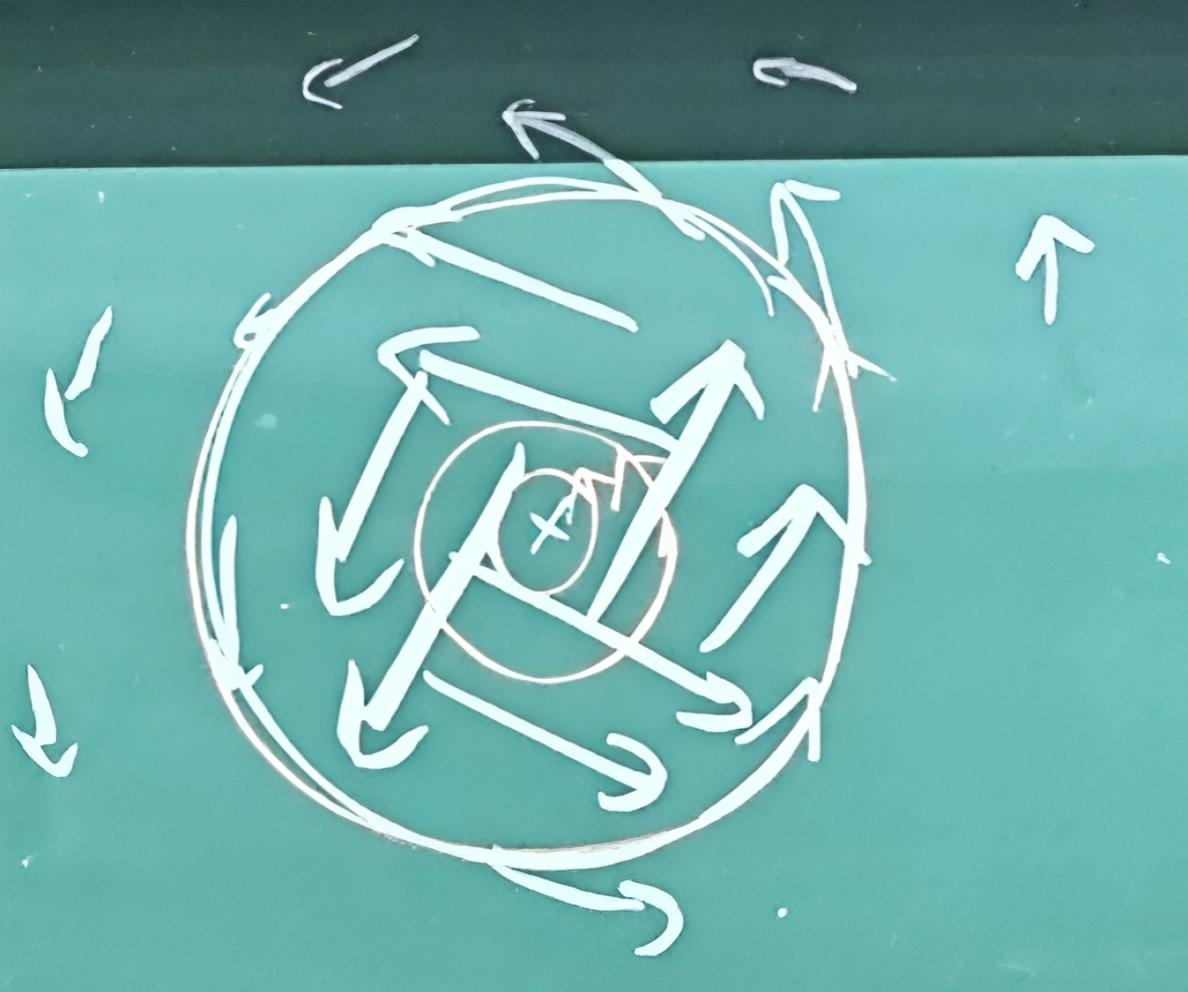
\includegraphics[height=3cm]{chapters/11/03/0204}
    \end{center}

    $$\oint\limits_{\substack{x^2+y^2=R^2\\\text{anti-clockwise}}}\frac{-y\overrightarrow{i}+x\overrightarrow{j}}{x^2+y^2}\,\mathrm{d}\overrightarrow{r}\xlongequal[y=R\sin t]{x=R\cos t}\int_0^{2\pi}\left(\frac{-R\sin t}{R^2},\frac{R\cos t}{R^2}\right)\cdot(-R\sin t,R\cos t)\,\mathrm{d}t=2\pi$$
\end{example}
\subsubsection{Green 定理}